% !Mode:: "TeX:DE:UTF-8:Main"
% arara: pdflatex
% arara: pdflatex
% xarara: convert: {density: 160, otheroptions: -dispose previous -delay 10 -loop 0, format: gif}
%magick -density 160 -delay 15 -loop 0 island.pdf island.gif
\documentclass{beamer}

\usepackage{tikzlings,tikzducks,xfp}
\usetikzlibrary{overlay-beamer-styles}
\setbeamertemplate{navigation symbols}{}
\tikzset{
  penguin1/.pic = {
   \begin{scope}[scale=.8,transform shape]
     \penguin;
  \end{scope}},
  penguin2/.pic = {
   \begin{scope}[scale=.6,transform shape]
     \penguin;
  \end{scope}},
  penguin3/.pic = {
   \begin{scope}[scale=.55,transform shape]
    \penguin
  \end{scope}
  },
  penguin4/.pic = {\begin{scope}[scale=0.7,transform shape]
  \penguin
  \end{scope}
  },
   snowman/.pic = {\begin{scope}[scale=0.7,transform shape]
  \snowman
  \end{scope}
  }
  }
\newcommand\penguini{0cm}
\newcommand\penguinii{0.3cm}
\newcommand\penguiniii{0cm}
\newcommand\penguiniv{0cm}
\newcommand\snowmanh{0.2cm}
\ExplSyntaxOn
\newcommand\myangle[1]{\fpeval{10*sin(#1)}}
\ExplSyntaxOff
\begin{document}
\begin{frame}<1->[plain,label=penguins]%%%%%%%%%%%%%%%%%%%%%%%%%%%%%%%%%%%%%%%%%%%%%%%%%
\begin{tikzpicture}[remember picture,overlay]
	
% Background image
\node[at=(current page.center)]{%
	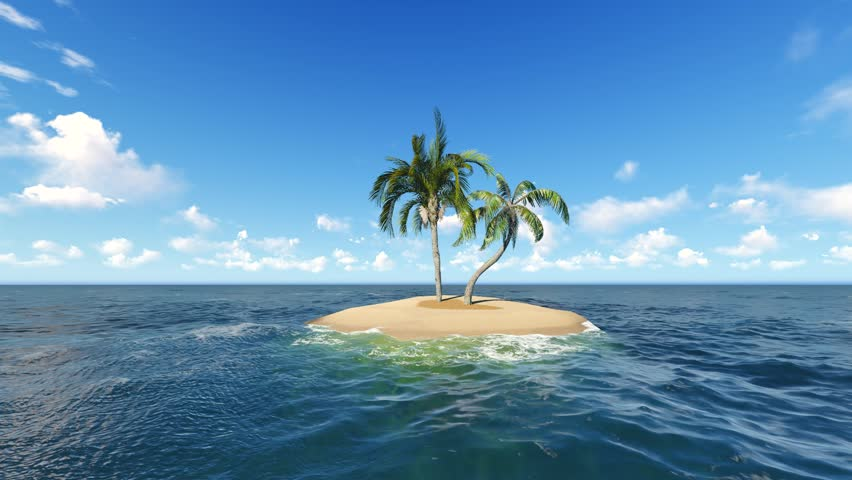
\includegraphics[height=1.05\paperheight,trim=2cm 2cm 2cm 2cm]{insel-mit-palme2}
};	

\only<50->{
	\node at ({5.4+0.5*sin(\value{page})},{28.8-0.0972*(\value{page}-50)}) {
\includegraphics[width=\paperwidth]{snowflakes}};
}

% Image credit of background
\node[at=(current page.south east),xshift=-6.6cm,yshift=0.2cm]{%
	\TINY\color{white}www.shutterstock.com};
\end{tikzpicture}

\vspace*{5cm}\hspace{1cm}
\foreach \x in {100,102,...,600}{%
\only<+>{%
\begin{tikzpicture}[overlay,baseline={(0,0)}]
\path(2.5,\penguini) pic[rotate=\myangle{\x}]{penguin1} -- (3.5,\penguinii)  pic [rotate=\myangle{\x}]{penguin2} -- (5.3,\snowmanh) pic[rotate=\myangle{\x}]{snowman}-- (6.3,\penguiniii) pic[rotate=\myangle{\x}]{penguin3} -- (8.3,\penguiniv) pic[rotate=\myangle{\x}]{penguin4};
\end{tikzpicture}}}

\end{frame}
\end{document} 